\documentclass{article}
\usepackage[utf8]{inputenc}
\usepackage{algorithm}
\usepackage{algpseudocode}
\usepackage{graphicx}
\usepackage{wrapfig}
\usepackage{geometry}
 \geometry{
 a4paper,
 total={170mm,257mm},
 left=20mm,
 top=20mm,
 }
\title{Drug Consumption: A Machine Learning Analysis of Marijuana 
and Other Drug Users}
\author{Priyanshi Aeron, Samantha Anthony, Zachary Hudgins, Tarini Ramesh}
\date{}

\begin{document}

\maketitle

\section{Introduction}

\section{Literature Review}

\section{Study Data}

\section{Methodology}
In order to answer our question and predict whether or not a participant was a marijuana user, we generated and tuned many different models. Because this is a supervised binary classification task, we modeled logistic classification, support vector machine, random forest, and a neural network due to their prominence and historic aptitude for binary classification tasks.
\subsection{Logistic Classification}
\subsection{Support Vector Machine}
\subsection{Random Forest}
The next model generated was a Random Forest model. A Random Forest is a powerful classifier that uses an ensemble of relatively uncorrelated decision trees which are then used as a whole to vote on which class each data point belongs to. To begin, we started from the bottom by building a single decision tree to get a baseline of how much our base model could stand to improve. This resulted in a base model accuracy of 0.848 and an AUC, or area under the receiver operating characteristic (ROC) curve, of 0.795. Next, we generated a base model for a random forest, which resulted in an accuracy of 0.8963 and AUC of 0.948. Since an AUC of 1.0 means perfect classification, and the random forest’s AUC was higher, it is easy to conclude that the random forest was better than just the single decision tree. However, even with these good accuracy and AUC measurements, the random forest could be improved by some parameter tuning. To tune the hyperparameters, the metric we were aiming to minimize was the out-of-bag (OOB) error, a standard measure of prediction error for random forests using bootstrapping, which averages prediction error on observations not used to generate the next tree. The hyperparameters that were tuned were the splitting criteria for each node, number of features for best split, maximum depth of the individual trees, and number of decision trees in the forest. Various values for each of these hyperparameters were tested against different random forests of many sizes. This hyperparameter tuning is displayed in the graphs and interpreted below.
\begin{figure}[htp]
    \centering
    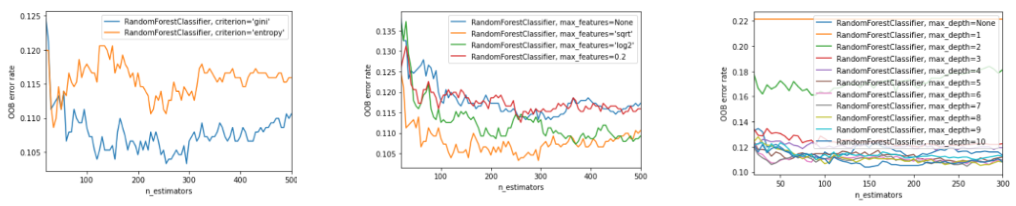
\includegraphics[width=12cm]{RF_hyperparameter_tuning.png}
    \label{fig:randforest}
\end{figure}

\noindent From the first graph, we can conclude that gini is the better criterion to minimize OOB error at larger values of the number of estimators used for the random forests. Additionally, the optimal maximum features parameter is the square root because it stabilizes to the lowest OOB error at the larger numbers of estimators. From the final graph, the maximum tree depths above around four all begin to converge to a very small OOB error, therefore the default parameter of no max depth was chosen because it produced the same results as the other depths. Finally, all of these values converge to low OOB errors around 150 to 300 decision trees, or estimators, in the forest, so the number of 250 decision trees was chosen due to it being in the range and not drastically increasing model computation time. After all the hyperparameter tuning, the model generated resulted in an accuracy of 0.915 and an AUC of 0.955. Therefore, the new tuned model was more accurate and had a larger AUC than the base models before, meaning it was a better model for the data.


\subsection{Neural Network}

\section{Results}
\begin{wrapfigure}{r}{7.4cm}
  \centering
  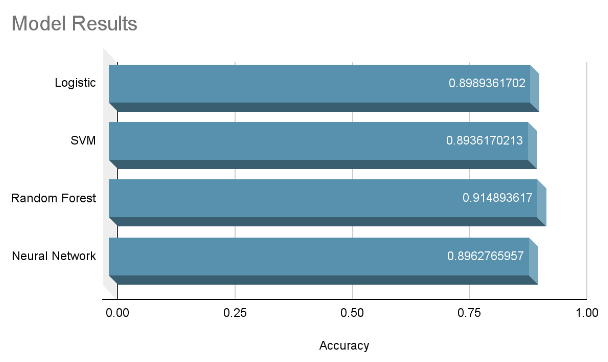
\includegraphics[height=3.7cm]{model_results.png}
\end{wrapfigure}
The models generated to answer our question were all decent models, as described above. They were all able to predict labels on the test set fairly well. This is further explored in the graph below of models by model accuracy on the test set. 
As evident in the Model Results figure, the model that produced the most accurate classification was the Random Forest. It is worth noting that all the models had around 0.90 accuracy and similarly high precision. However, due to its higher accuracy and in-depth analysis features, the Random Forest model was chosen as our best model to solve this task.
\begin{figure}[htp]
\centering
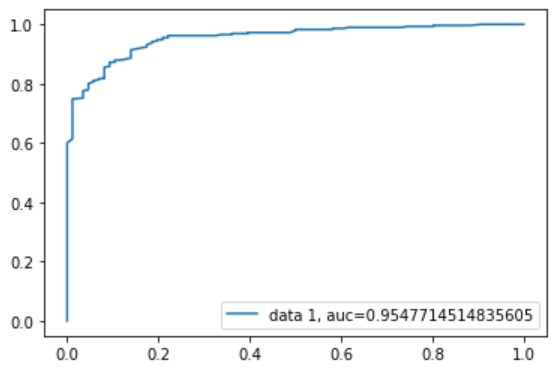
\includegraphics[width=.3\textwidth]{rf_auc_curve.png}\hfill
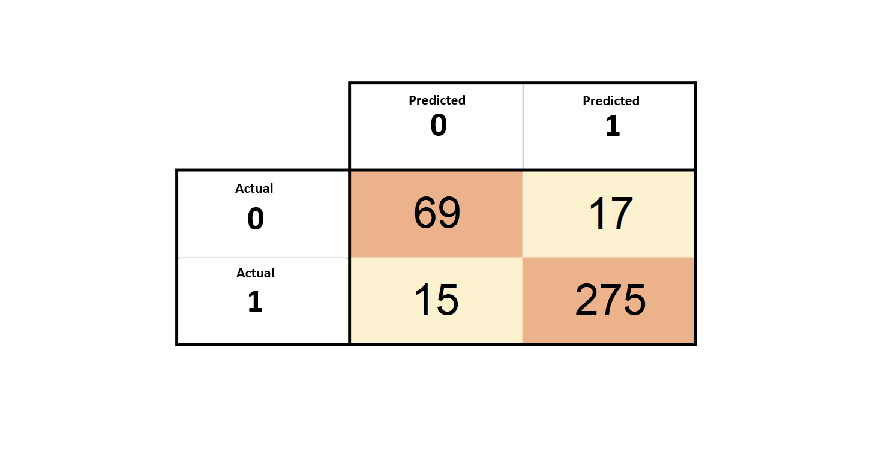
\includegraphics[width=.3\textwidth]{rf_conf_matrix.png}\hfill
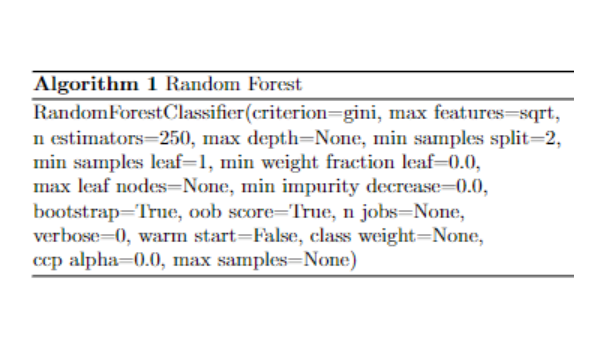
\includegraphics[width=.4\textwidth]{rf_algorithm.png}
\end{figure}

\noindent After testing the optimized model, the random forest resulted in an AUC of 0.955 and an accuracy of 0.915 on the test set. The ROC curve, confusion matrix, and algorithm are displayed above, in order. Following the creation and verification of that model, we started looking into how the random forest was able to conclude who was a marijuana user vs participants who have never used it in their lives. To do so, we looked at feature importance.

According to the model, the most important determining factor of whether or not a participant was a marijuana user was if they also used nicotine. This makes sense given the previously found correlations between marijuana users and smokers. This relationship could be due to the fact that these drugs are accessible, however other highly accessible drugs like alcohol and caffeine were not a huge predictor in marijuana use. What is more likely is that nicotine and marijuana have interactive effects on the brain when used together. 
Next, we investigated if a certain schedule of drug, as determined by the United States Drug Enforcement Administration, would provide any insight into marijuana users. These results are color coded by schedule in the graph on the left above. Marijuana is a schedule 1 drug, so people claiming it was a gateway drug would expect other high schedule drugs to be very large indicators of marijuana use. However, the main predictors of marijuana use are decently split between legal, non-scheduled drugs and schedule 1 and 2 drugs. Therefore, one cannot conclude that marijuana use leads to other harder drug use, such as Meth or Heroin.
By looking at feature importance in relation to the type of drug, we were able to generate the above graph on the right. Marijuana is a hallucinogen and stimulant, therefore one would expect marijuana use to lead to other hallucinogenic drug use. As evident in the figure, there is a high correlation between marijuana use and other hallucinogens and stimulants, such as Nicotine, Mushrooms, and Cocaine.
	
Overall, we were able to generate a highly successful random forest model that is able to predict whether or not someone is a marijuana user with over 90 percent accuracy. By exploring this model, we were also able to show that marijuana use is highly related to nicotine, a fact supported by previous research. We were not able to show that marijuana use leads to other hard drug use, indicating that marijuana may not be the dangerous gateway drug that a lot of society was led to believe that it is. Finally, we were able to show that users of marijuana tended to use and seek out similar drugs such as other hallucinogens and stimulants like Mushrooms. 


\section{Future Research}

\section{Conclusion}

\end{document}
